\documentclass[tikz]{standalone}

\usepackage[outline]{contour}
%\usepackage{tikz}

\contourlength{0.35pt}

% tikz setup
\usetikzlibrary{automata, positioning, arrows}

\tikzstyle{every path} = [draw=black]

\tikzstyle{every state} = [fill=white]

\tikzset{%
    ->,
    >=stealth',
    node distance=2cm,
    initial text=$ $,
}

\tikzset{%
    every edge/.style={%
        text=white,
    }
}

\newcommand{\nodestroke}[1]{\contour{black}{#1}}

\begin{document}
    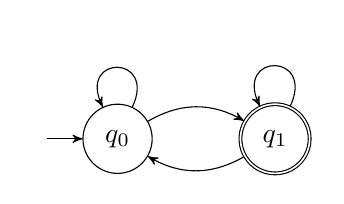
\begin{tikzpicture}
        \node[state, initial] (q0) {$q_0$};
        \node[state, accepting, right of=q0] (q1) {$q_1$};

        \draw (q0) edge[above, in=115, out=65, looseness=5] node {$a$} (q0)
        (q0) edge[above, bend left] node {$b$} (q1)
        (q1) edge[above, in=115, out=65, looseness=5] node {$b$} (q1)
        (q1) edge[above, bend left] node {$a$} (q0)
        ;
    \end{tikzpicture}
\end{document}